\paragraph{Corollaire}
Si $f(x) \neq 0$ et $f(b) \neq 0$ avec $a, b$ de signes différents dans $\mathbb{R}$, alors il existe un $c \in ]a, b[$ tel que $f(x) = 0$

\paragraph{Corollaire}

\begin{align*} 
	f & \text{fonction continue} \\
	f & : \mathbb{R} \rightarrow \mathbb{R}
\end{align*}

tel que $\lim_{x\to +\infty} f(x) = +\infty$ et $\lim_{x\to -\infty} f(x) = -\infty$ alors f est surjective.

\paragraph{Idée de démonstration}

Ramener à un intervalle "bornée", de type $[a, b] \in \mathbb{R}^2, a < b$. ~\\
Soit $y \in \mathbb{R}$, et $x_1, x_2 \in \mathbb{R}$ tel que $x_1 < x_2$ et $f(x_1) = y-1$ et $f(x_2) = y+1$. On cherche à prouver qu'il existe au moins un antécédent.

$\lim_{x\to +\infty} f(x) = +\infty$ donc $f(x) \geq y + 1$ pour x assez grand.

$\lim_{x\to -\infty} f(x) = -\infty$ donc $f(x) \leq y - 1$ pour x assez petit.
On applique le théorème des valeurs intermédiaire à $f_{|[x_1, x_2]} : [x_1, x_2] \rightarrow \mathbb{R}$ et $f_{|[x_1, x_2]}$ est bien continue. 

Comme $f(x_1) \leq y-1 < y < y+1 \leq f(x_2)$
~\\
D'où il existe $x \in [x_1, x_2]$ tel que $f(x) = y$.
\paragraph{Corollaire} 
$f : I \rightarrow \mathbb{R}$, continue sur $I \in \mathbb{R}$, alors $f(I)$ est un intervall.

\section{Continuité et extremum}

\paragraph{Définition} Soit $E \subset \mathbb{R}$. ~\\
\begin{itemize}
	\item On dit que x est le \ul{minimum} de E, si pour tout élément de $x' \in E$, $x' \geq x$
	\item On dit que x est le \ul{maximum} de E, si pour tout élément de $x' \in E$, $x' \leq x$
	\item Un \ul{extremum} est un minimum ou un maximum.
\end{itemize}

\paragraph{Remarque} Le maximum et le minimum sont unique.

\paragraph{Théorème} Soit $f:[a, b] \rightarrow \mathbb{R} (a < b)$, continue. ~\\
L'image de f admet un minimum et un maximum.

\paragraph{Remarque} de manière équivalente : Minimum ~\\
$\exists y \in Im(f), \forall y' \in Im(f), y' \geq y$ (ou y est le minimum)
~\\
$\exists x_{min} \in [a, b], \forall x' \in [a, b], f(x') \geq f(x_{min})$ (avec $y = f(x_{min})$ et $y'=f(x')$)
~\\
~\\
Pour le maximum :  $\exists x_{max} \in [a, b], \forall x' \in [a, b], f(x') \leq f(x_{max})$ ($f(x_{max})$ le maximum de $Im(f)$)
~\\

Dans ces exemples, y est forcément unique (dans le cas du minimum ou du maximum) mais il peut y avoir plusieurs antécédents (plusieurs $x_{min}$ et $x_{max}$)

\paragraph{Exemple} $\sin : [0, 4\pi] \rightarrow [-1, 1]$ ~\\
Le minimum de $\sin_([0, 4\pi])$ est -1. Il est atteint en $\frac{3\pi}{2}$ et $\frac{7\pi}{2}$.

\paragraph{Remarque}

\begin{wrapfigure}[5]{r}{0pt}
	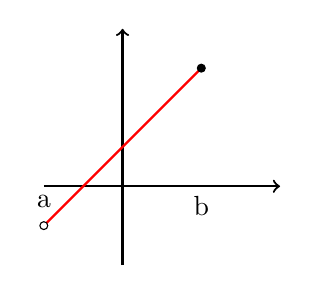
\begin{tikzpicture}
		\draw[->, thick] (-1, 0) -- (2, 0);
		\draw[->, thick] (0, -1) -- (0, 2);
		\draw[red, thick] (-1, -0.5) -- (1, 1.5);
		\draw[fill=white] (-1, -0.5) circle (0.05);
		\draw[fill=black] (1, 1.5) circle (0.05);

		\node at (-1, 0) [below] {a};
		\node at (1, 0) [below] {b};
	\end{tikzpicture}
\end{wrapfigure}
2 hypothèses. Pour avoir un maximum ou un minimum, $[a, b]$ doit etre un intervalle \ul{ferme} et \ul{borne}. Par exemple, Le minimum n'est pas atteint sur $]a, b]$ De meme, sur $[a, b[$ pour le maximum.

		\paragraph{Corollaire} supposons $f : \mathbb{R} \rightarrow \mathbb{R}$ continue. ~\\
		Si $\lim_{x \to -\infty} f(x) = +\infty$ et $\lim_{x \to +\infty} f(x) = +\infty$, alors f admet un minimum mais pas de maximum.

		\paragraph{Idée de démonstration}
\begin{tikzpicture}[scale=0.5]
	\clip (7, 7) rectangle (-5, -0.9);
	\draw[domain=-3:3, red] plot(\x, {\x * \x});
	\node at (2, 3) [red, right] {$x \mapsto x^2$};
	\draw[->, thick] (-3, 0) node [below] {a} -- (3, 0) node [below] {b};
	\draw[->, thick] (0, 0) -- (0, 7);
\end{tikzpicture}

Cette fonction admet un minimum (0) mais jamais de maximum.

\paragraph{Corollaire} $f : [a, b] \rightarrow \mathbb{R}$ continue. ~\\
Si pour tout $x \in [a, b], f(x) > 0$ alors le minimum de $Im(f) > 0$,~\\
c'est à dire $\exists m > 0, \forall x \in [a, b], f(x) \geq m > 0$

\section{Fonctions réciproques}

\paragraph{Théorème} $f : I \rightarrow \mathbb{R}$, continue et strictement monotone.
\begin{enumerate}
	\item $f(I)$ est un intervall
	\item $f$ est bijective sur $J$
	\item $f^{-1}$  est continue et strictement monotone, avec le meme sens de variations que f.
	\item Les graphs de $f$ et $f^{-1}$ sont symétriques par rapport à la première bisectrice $\Delta y=x$
\end{enumerate}

Exemple $\sin [-\frac{\pi}{2}, \frac{\pi}{2}] \rightarrow [-1, 1]$ est continue et strictement croissante.

\begin{wrapfigure}[3]{l}{0pt}
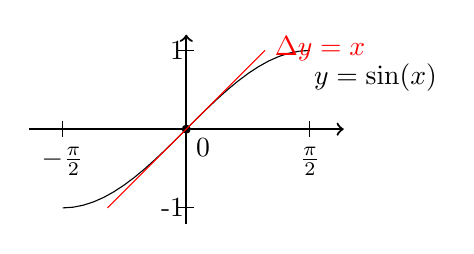
\begin{tikzpicture}

\draw[->, thick, black] (0, -1.2) -- (0, 1.2);
\draw[->, thick] (-2, 0) -- (2, 0);
\draw[domain=-1.57:1.57] plot (\x, {sin(\x r)});
\draw[fill=black] (0, 0) circle (0.05);
\foreach \x/\text in {
	-1.57/$-\frac{\pi}{2}$,
	1.57/$\frac{\pi}{2}$}
\draw[] (\x, 0.1) -- (\x, -0.1) node[below, fill=white] {\text};
\node[right] at (1.5, 0.65) {$y=\sin(x)$};

\draw[] (-0.1, 1) -- (0.1, 1) node [xshift=-0.1, left] {1};
\draw[] (-0.1, -1) -- (0.1, -1) node [xshift=-0.1, left] {-1};
\node at (0, 0) [below right] {0};
\draw[red] (-1, -1) -- (1, 1) node [yshift=0.5, right] {$\Delta y=x$};

\end{tikzpicture}
\end{wrapfigure}
Donc f est bijective, c'est à dire $f^{-1} : [-1, 1] \rightarrow [-\frac{\pi}{2}, \frac{\pi}{2}]$ existe et $f^{-1}$ vaut arcsinus. ~\\
$arcsin : [-1, 1] \rightarrow [-\frac{\pi}{2}, \frac{\pi}{2}]$ est continue et strictement croissante.

~\\
~\\
~\\
~\\

\begin{center}
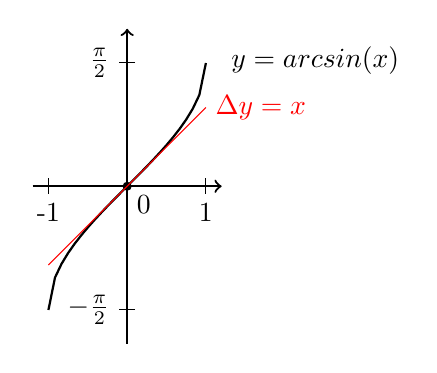
\begin{tikzpicture}

\draw[->, thick, black] (0, -2) -- (0, 2);
\draw[->, thick] (-1.2, 0) -- (1.2, 0);
\draw[thick, domain=-1:1] plot (\x, {asin(\x)/360*2*pi});
\node[right] at (1.2, 1.6) {$y=arcsin(x)$};
\draw[fill=black] (0, 0) circle (0.05);
\foreach \x/\text in {
	-1.57/$-\frac{\pi}{2}$,
	1.57/$\frac{\pi}{2}$}
\draw[] (0.1, \x) -- (-0.1, \x) node[left, fill=white] {\text};

\draw[] (1, 0.1) -- (1, -0.1) node [below] {1};
\draw[] (-1, 0.1) -- (-1, -0.1) node [below] {-1};
\node at (0, 0) [below right] {0};

\draw[red] (-1, -1) -- (1, 1) node [right] {$\Delta y=x$};

\end{tikzpicture}
\end{center}

Exemple $\cos [0, \pi] \rightarrow [-1, 1]$ est continue et strictement croissante.

\begin{wrapfigure}[3]{l}{0pt}
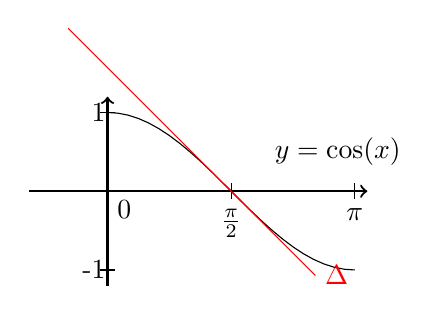
\begin{tikzpicture}

\draw[->, thick, black] (0, -1.2) -- (0, 1.2);
\draw[->, thick] (-1, 0) -- (3.3, 0);
\draw[domain=0:3.14] plot (\x, {cos(\x r)});
\foreach \x/\text in {
	1.57/$\frac{\pi}{2}$,
	3.14/$\pi$}
\draw[] (\x, 0.1) -- (\x, -0.1) node[below] {\text};

\draw[] (-0.1, 1) -- (0.1, 1) node [xshift=-0.1, left] {1};
\draw[] (-0.1, -1) -- (0.1, -1) node [xshift=-0.1, left] {-1};
\node at (0, 0) [below right] {0};

\draw[red] (-0.5, 2.07) -- (2.64, -1.07) node [right] {$\Delta$};
\node[right] at (2, 0.5) {$y=\cos(x)$};

\end{tikzpicture}
\end{wrapfigure}
Donc f est bijective, c'est à dire $f^{-1} : [-1, 1] \rightarrow [0, \pi]$ existe et $f^{-1}$ vaut arccosinus. ~\\
$arccos : [-1, 1] \rightarrow [0, \pi]$ est continue et strictement croissante.

~\\
~\\
~\\
~\\

\begin{center}
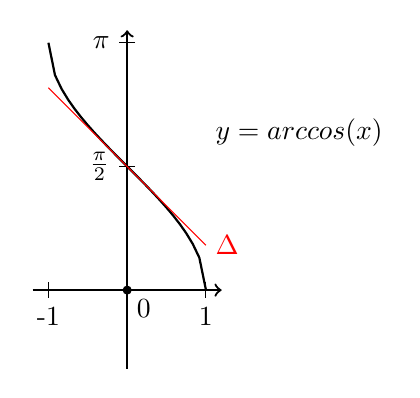
\begin{tikzpicture}

\draw[->, thick, black] (0, -1) -- (0, 3.3);
\draw[->, thick] (-1.2, 0) -- (1.2, 0);
\draw[thick, domain=-1:1] plot (\x, {acos(\x)/360*2*pi});
\draw[fill=black] (0, 0) circle (0.05);
\foreach \x/\text in {
	1.57/$\frac{\pi}{2}$,
	3.14/$\pi$}
\draw[] (0.1, \x) -- (-0.1, \x) node[left] {\text};

\draw[] (1, 0.1) -- (1, -0.1) node [below] {1};
\draw[] (-1, 0.1) -- (-1, -0.1) node [below] {-1};
\node at (0, 0) [below right] {0};

\draw[red] (-1, 2.57) -- (1, 0.57) node [right] {$\Delta$};
\node[right] at (1, 2) {$y=arccos(x)$};

\end{tikzpicture}
\end{center}

\newpage

\paragraph{Exemple} $\tan : ]\frac{-\pi}{2}, \frac{\pi}{2}[ \rightarrow \mathbb{R}$ est continue et strictement croissante, donc sa fonction reciproque est:
$arctan : \mathbb{R} \rightarrow ]\frac{-\pi}{2}, \frac{\pi}{2}[$ aussi.

\begin{wrapfigure}[3]{l}{0pt}
\begin{tikzpicture}

	\clip (-2, 3) -- (4, 3) -- (4, -3) -- (-2, -3) --cycle;

\draw[->, thick, black] (0, -3) -- (0, 3);
\draw[->, thick] (-2, 0) -- (2, 0);
\draw[domain=-1.56:1.56] plot (\x, {tan(\x r)});
\draw[fill=black] (0, 0) circle (0.05);
\foreach \x/\text in {
	-1.57/$-\frac{\pi}{2}$,
	1.57/$\frac{\pi}{2}$}
\draw[] (\x, 0.1) -- (\x, -0.1) node[below, fill=white] {\text};

\draw[] (-0.1, 1) -- (0.1, 1) node [left] {1};
\draw[] (-0.1, -1) -- (0.1, -1) node [left] {-1};
\node at (0, 0) [below right] {0};
\draw[red] (-1, -1) -- (1, 1) node [right] {$\Delta$};
\node[right] at (1, 1.5) {$y=\tan(x)$};

\end{tikzpicture}
\end{wrapfigure}
Donc f est bijective, c'est à dire $f^{-1} : \mathbb{R} \rightarrow [-\frac{\pi}{2}, \frac{\pi}{2}]$ existe et $f^{-1}$ vaut arctangeante. ~\\
$arctan : \mathbb{R} \rightarrow [-\frac{\pi}{2}, \frac{\pi}{2}]$ est continue et strictement croissante.

~\\
~\\
~\\
~\\

\begin{center}
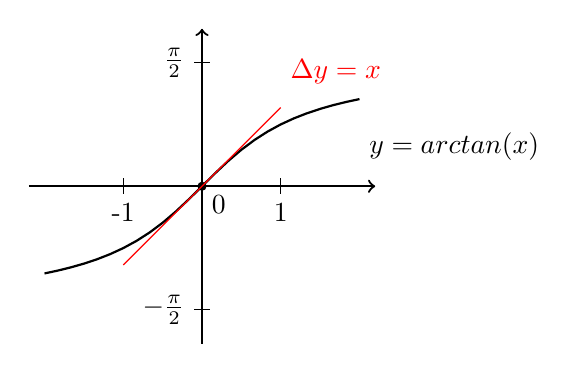
\begin{tikzpicture}

\draw[->, thick, black] (0, -2) -- (0, 2);
\draw[->, thick] (-2.2, 0) -- (2.2, 0);
\draw[thick, domain=-2:2] plot (\x, {atan(\x)/360*2*pi});
\draw[fill=black] (0, 0) circle (0.05);
\foreach \x/\text in {
	-1.57/$-\frac{\pi}{2}$,
	1.57/$\frac{\pi}{2}$}
\draw[] (0.1, \x) -- (-0.1, \x) node[left, fill=white] {\text};

\draw[] (1, 0.1) -- (1, -0.1) node [below] {1};
\draw[] (-1, 0.1) -- (-1, -0.1) node [below] {-1};
\node at (0, 0) [below right] {0};

\draw[red] (-1, -1) -- (1, 1);
\node[right, red] at (1, 1.45) {$\Delta y=x$};
\node[right] at (2, 0.5) {$y=arctan(x)$};

\end{tikzpicture}
\end{center}

\paragraph{Exemple} ~\\
$
\left\{
\begin{array}{c}
	n \in \mathbb{N}^* \\
	x \mapsto x^n
\end{array}
\right.$ est continue sur $\mathbb{R}$.
Elle est strictement croissante sur $\mathbb{R}^+$ si n est pair. ~\\
Elle est donc bijective : $\left\{
	\begin{array}{rcl}
		x & \mapsto & x^{\frac{1}{n}} \\
		\mathbb{R}^+& \rightarrow &\mathbb{R}^+
	\end{array}
		\right.
		$
elle est strictement croissante sur $\mathbb{R}$ si n est impair.
Reciproque $\left\{
	\begin{array}{rcl}
		x & \mapsto& x^{\frac{1}{n}} \\
		\mathbb{R} &\rightarrow& \mathbb{R}
	\end{array}
	\right.
		$
